\documentclass[svgnames]{beamer}

\usepackage[T1]{fontenc}
\usepackage{graphicx}
\usepackage{longtable}
\usepackage{wrapfig}
\usepackage{rotating}
\usepackage[normalem]{ulem}
\usepackage{amsmath}
\usepackage{amssymb}
\usepackage{capt-of}
\mode<beamer>{\usetheme{Berlin}}
\usecolortheme {dolphin}


\usepackage[x11names]{xcolor}

\usepackage{mathrsfs}
\usepackage{tikz-cd}

\usepackage{fontspec}
\setmonofont{FreeMono}
\setmainfont{FreeSerif}

\usepackage{unicode-math}

\usepackage[dvipsnames]{xcolor}

\usepackage{amsthm}
\usepackage{thmtools}

\usepackage{minted}
\usemintedstyle{tango}


\definecolor{MyTOCColor}{RGB}{90, 150, 220}
\definecolor{MyTOCColor2}{RGB}{31, 31, 31} 
\definecolor{MyTOCColor3}{RGB}{255, 255, 255}

\setbeamercolor{structure}{fg=MyTOCColor}
\setbeamercolor{background canvas}{bg=MyTOCColor2}
\setbeamercolor{normal text}{fg=MyTOCColor3}  

\setbeamercolor{item}{fg=MyTOCColor}
\setbeamercolor{title}{fg=MyTOCColor3}
\setbeamercolor{frametitle}{fg=MyTOCColor3}

\newcommand{\Z}{\mathbf{Z}}
\newcommand{\Q}{\mathbf{Q}}
\newcommand{\R}{\mathbf{R}}
\newcommand{\C}{\mathbf{C}}
\newcommand{\F}{\mathbf{F}}
\newcommand{\N}{\mathbf{N}}

\newcommand{\LL}{\mathscr{L}}
\newcommand{\pp}{\mathbf{p}}
\newcommand{\xx}{\mathbf{x}}
\newcommand{\yy}{\mathbf{y}}
\newcommand{\vv}{\mathbf{v}}
\newcommand{\ww}{\mathbf{w}}
%%--------------------------------------------------------------------------------
\author{Sahan Wijetunga}
\date{2025-07-24}
\title{Formalization in Lean}
\hypersetup{
 pdfauthor={Sahan Wijetunga},
 pdftitle={Formalization and Finite Algebra},
 pdfkeywords={modelling},
 pdfsubject={},
 pdfcreator={Emacs 31.0.50 (Org mode 9.7.11)}, 
 pdflang={English}}
\usepackage{biblatex}

\begin{document}

\maketitle
\begin{frame}{Outline}
\tableofcontents
\end{frame}

\setbeamertemplate{blocks}[rounded][shadow=true]


\section{Introduction}
\begin{frame}{What is Formalization?}
\centering
``Expressing mathematics (objects, arguments) in a format that a computer can handle and interact with rigorously.'' - Kevin Buzzard
\end{frame}

\begin{frame}{Benefits of Formalization}
\centering
\begin{itemize}
    \item Finding Mistakes
    \item Allowing large scale collaboration
    \begin{itemize}
            \item Equational theories project
        \item Public formalization projects
        \item Base productivity shrunk by a large constant factor
    \end{itemize}
    \item Pedagogical benefits 
\end{itemize}
\end{frame}

\section{Types}

\subsection{Type Theory in Lean}
\begin{frame}{Lean works using Type Theory}
\begin{itemize}[<+->]
    \item Every object has an associated \textit{Type}
    \begin{itemize}[<+->]
        \item $\sqrt 2: \mathbb R$ 
        \item $1: \mathbb N$ 
        \item $\text{id}: \mathbb Q \to \mathbb Q$ 
        \item $\mathbb N: \text{Type}$ 
    \end{itemize}
    \item Definitions must be created with types specified.
    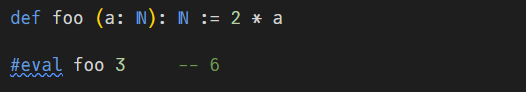
\includegraphics[width=0.75\linewidth]{image.png}
    \item Types can be omitted with implicit notation.
    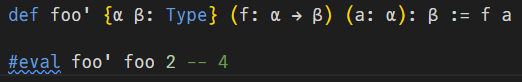
\includegraphics[width=0.75\linewidth]{image2.png}
\end{itemize}
\end{frame}
\subsection{Type Classes}
\begin{frame}{Type Classes in Lean}
\begin{itemize}[<+->]
    \item Implicit \{\} notation allows you to avoid giving types explicitly.
    \item Type classes allows you to have much more inferred from context
    \item 
\begin{figure}
    \centering
    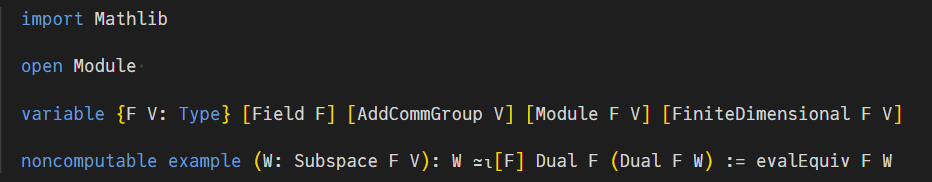
\includegraphics[width=0.75\linewidth]{image4.png}
\end{figure}
    \item \begin{figure} \centering 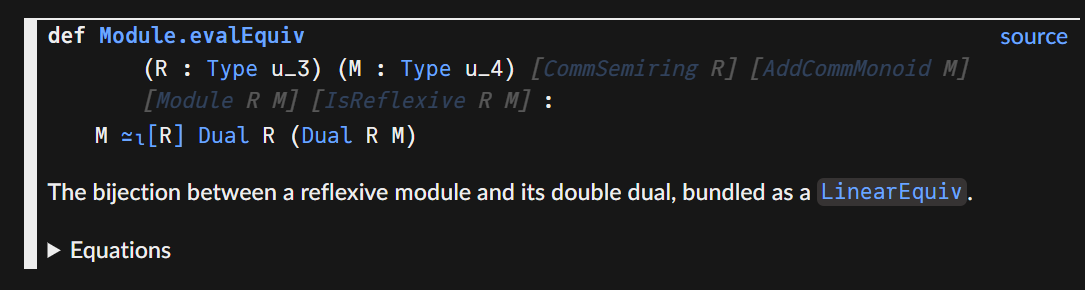
\includegraphics[width=0.75\linewidth]{image5.png}\end{figure}
\end{itemize}
\end{frame}

\begin{frame}{Issues with Type Classes}
\begin{itemize}[<+->]
    \item Hard to see whats going on
    \item Slow compile times
    \item \begin{figure}
    \centering
    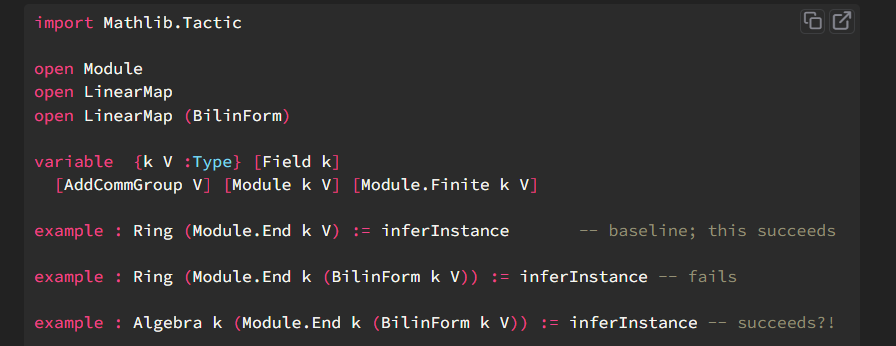
\includegraphics[width=1\linewidth]{image6.png}
\end{figure}
\end{itemize}
\end{frame}

\begin{frame}{Diamonds}
\begin{itemize}[<+->]
    \item Suppose A has an instance for B and C, which both have instances for D. Then A has two instances for D. Which to choose? 
    \item 
\begin{figure}
    \centering
    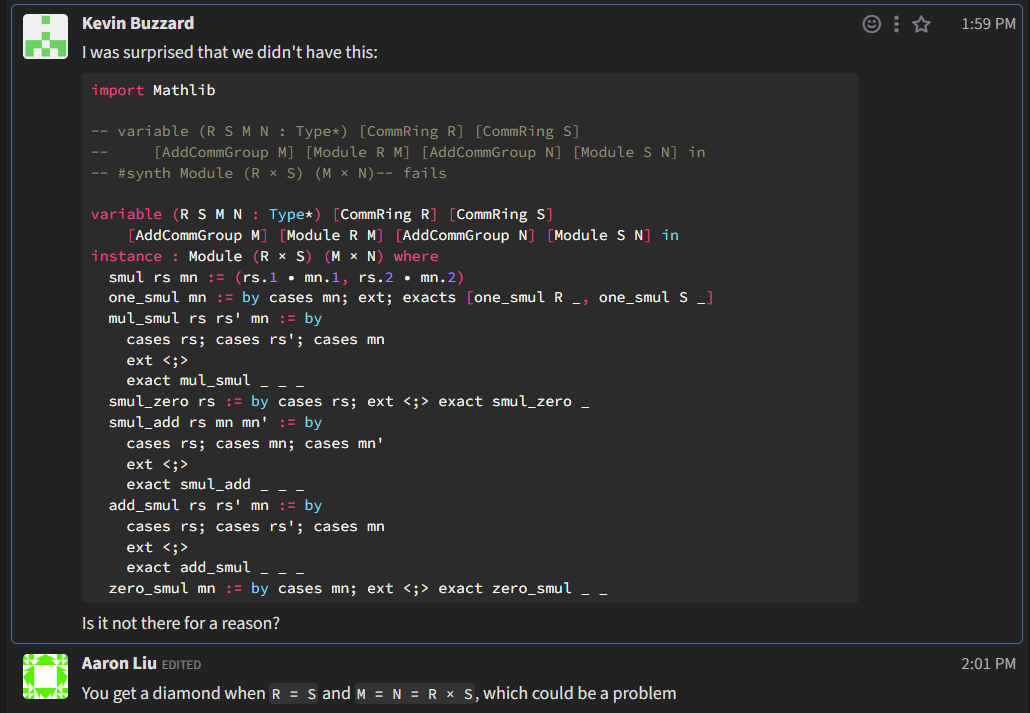
\includegraphics[width=0.75\linewidth]{image7.png}
\end{figure}
\end{itemize}
\end{frame}

\section{Definitions}

\begin{frame}
\centering
\Large
Proofs in Lean are guaranteed to be correct. 

$ $

$ $

$ $

\pause But what if your definitions are wrong?
\end{frame}

\begin{frame}{Orthogonal Complement}
\begin{itemize}[<+->]
    \item We say $V$ is the internal direct sum of $W_1$ and $W_2$ with respect to a bilinear form $B: V \times V \to F$ if 
\begin{itemize}[<+->]
    \item $W_1$ and $W_2$ are \textit{orthogonal}, i.e. that $B(w_1,w_2)=0$ for all $w_1 \in W_1$ and $w_2 \in W_2$,
    \item $W_1+W_2=V$,
    \item $W_1 \cap W_2=0$. 
    \end{itemize}
    \item This doesn't force $W_2$ orthogonal to $W_1$! \pause I.e, the form is only to be block upper triangular rather than block diagonal. 
    \pause \item Explicitly checking examples in Lean, and immediately proving compatibility results with similar theorems helps avoid this
\end{itemize}

\end{frame}

\subsection{Equality}

\begin{frame}{Forced Implementation Choice}
\begin{itemize}[<+->]
    \item Exact definition $p$ of an object not viewed with much importance in math, as we can just prove $p \iff q$ and then use $q$ everywhere
    \item Lean forces us to pick a privileged definition
    \item A basis in Lean internally is an $F$-linear isomorphism $V \simeq F^\alpha$
    \item $F$-linear isomorphisms are themselves implemented as maps $V \to W$ and $W \to V$ which are inverses. 
    \item In the REU, I formalized Hyperbolic bilinear forms using a basis and a predicate,\pause whereas the Mathlib one uses an isomorphism to $V^* \times V$
    \item Allowing computations or not
\end{itemize}
\end{frame}

\begin{frame}{Canonical Isomorphism}
\begin{itemize}[<+->]
    \item There is an obvious isomorphism $X \times (Y \times Z) \simeq(X \times Y) \times Z $ to where we just write $=$ directly. 
    \item Often in algebra we just write $=$ for canonical isomorphism or even for definitions (via universal properties), like with $A \otimes_R B$. 
    \item Limits practical freedom and forces people to be more explicit in choices
\end{itemize}

\end{frame}

\subsection{Finding Internals}

\begin{frame}{Quadratic Forms Extension by Scalars}
\begin{itemize}[<+->]
    \item A given quadratic form $\phi: V \to F$ can be extended to one $A \otimes_F V \to A$ for $F$-algebras $A$. 
    \item The Lean implementation of this goes through Bilinear forms, forcing $2 \neq 0$ in $F$. 
    \item Fairly easy to find what is exactly needed/true for definitions from Mathlib
    \begin{itemize}[<+->]
        \item Improvement to traditional textbooks
    \end{itemize}
\end{itemize}
\end{frame}

\begin{frame}{Quadratic Forms Extension by Scalars}

 \begin{figure}
    \centering
    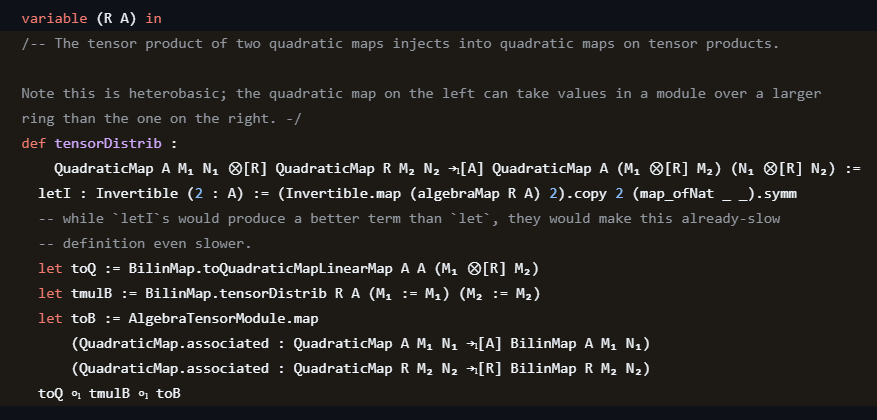
\includegraphics[width=1\linewidth]{image8.png}
\end{figure}
\pause Ended up using the external framework of theorems instead
\end{frame}


\section{Lean}

\begin{frame}{Lean}

\vspace{1cm} 

\begin{columns}[t] 
  \column{0.5\textwidth}
  \textbf{Current Issues}
  \begin{itemize}[<+->]
    \item Strict Definitions
    \item \textit{Dependent} Type Theory
    \item Universe issues (rarely)
    \item Manually using type classes not automatically instantiated to avoid diamonds
    \item Mathlib having large gaps
  \end{itemize}
    
  \column{0.5\textwidth}
  \pause \textbf{To be Improved On:}
  \begin{itemize}[<+->]
      \item Tooling
      \begin{itemize}[<+->]
          \item Better Tactics
          \item AI Usage
      \end{itemize}
      \item The Math
  \end{itemize}
\end{columns}


\end{frame}

\begin{frame}{Contributing to Mathlib}
\begin{itemize}[<+->]
    \item Code to be ported to Mathlib over time, cleaning portions at a time
    \item In the form of ``pull requests''
    \item Results to be ported over: 
    \begin{itemize}[<+->]
        \item Bilinear Form Isometries (Isomorphisms)
        \item Notion of degree over polynomial modules, and the surrounding theory
        \item Quotients of bilinear and quadratic forms
        \item Surrounding theory for Hyperbolic Spaces
        \item Compatibility of quadratic and bilinear forms and degree notions with extensions of scalars by the polynomial ring
        \item Cassels-Pfister Theorem: The values taken by the extension of a quadratic map $\phi: V \to F$ to $V(X) \to F(X)$ that are in $F[X]$ are taken by the extension $V[X] \to F[X]$. 
    \end{itemize}
\end{itemize}
\end{frame}

\begin{frame}{Current State}
\begin{itemize}[<+->]
    \item The Symmetric algebra of a vector space has been formalized, however the grading on it has not (though being actively discussed). 
    \begin{itemize}[<+->]
        \item This blocks progress on constructing extension by scalars in characteristic 2
    \end{itemize}
    \item Fermat's Last Theorem: Current effort to formalize led by Kevin Buzzard
    \item The polynomial Freiman–Ruzsa conjecture was proved in 2023 by Tim Gowers, Ben Green, Freddie Manners, and Terry Tao, and has been formalized in Lean. 
\end{itemize}
\end{frame}

\begin{frame}
	    \begin{center}
	        \textbf{Thank you!}\\
	        
	        Special thanks to Dr. George McNinch, the VERSEIM REU, and National Science Foundation for their support under REU Site grant DMS-2349058.”
         \bigbreak
         \LARGE
       
	    \end{center}
\end{frame}

\end{document} 